\section{Structured Assurance Case Metamodel}
\label{sec:sec2}
The \textit{Structured Assurance Case Metamodel} (SACM) is standardised by the Object Management Group (OMG). The intention of the metamodel is to promote model-based approach in the process of \textit{System Assurance}, which is currently a manual approach with (mostly) computer unfriendly artefacts as results (i.e. Assurance Cases). SACM is created to support structural argumentation approaches such as the \textit{Goal Structuring Notation} (GSN) and \textit{Claims, Arguments and Evidence} (CAE). 

SACM captures not only fundamental concepts in the process of \textit{System Assurance} such as \textit{Claim}s and the relationships between \textit{Claim}s, it also captures concepts such as \textit{Artifact}s and \textit{Terminologi}es, in the sense that supporting evidence and information involved in the argument can be expressed in greater precision. 

In addition, SACM promotes \textit{modularity}, in the sense that assurance cases are organised in packages, which in turn organise argumentations, evidence and terminologies in corresponding packages. SACM also promotes \textit{openness} in the sense that external information (such as external models and/or documents) can be linked via the facilities provided in SACM. This section discusses in detail the facilities provided in SACM and how they can be used in \textit{System Assurance}.

\begin{figure}
	\centering
	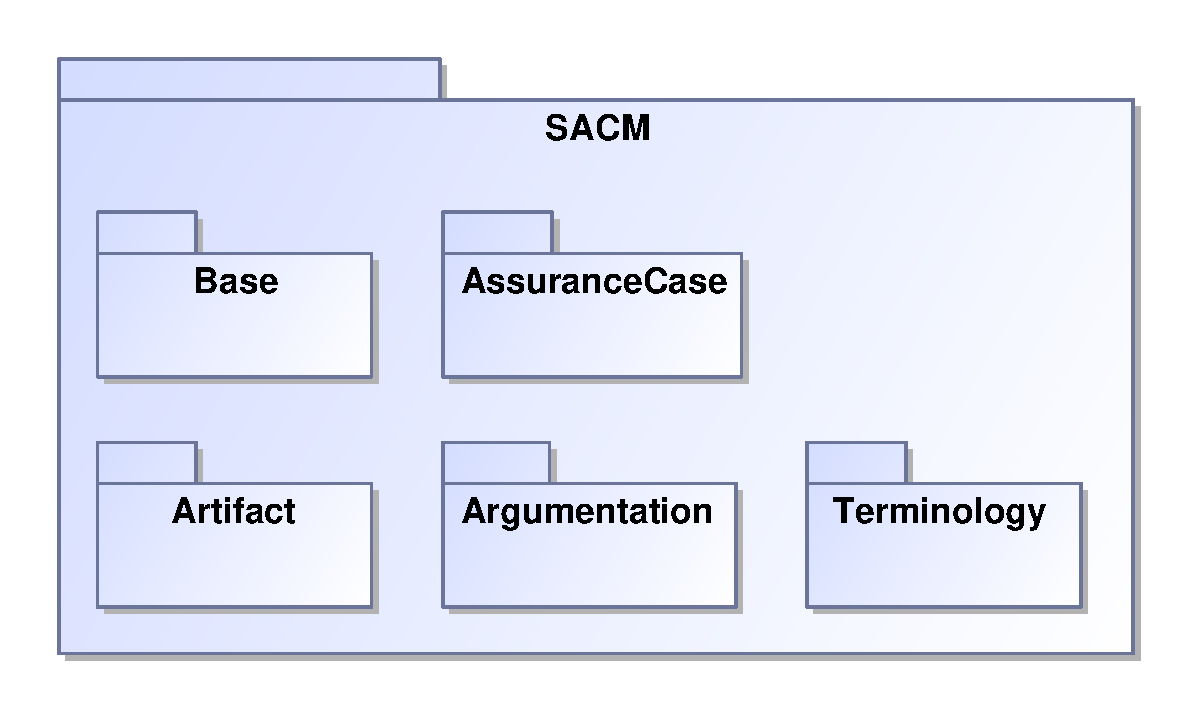
\includegraphics[width=0.6\linewidth]{fig/Overview.eps}
	\caption{Packages of SACM}
	\label{fig:overview}
\end{figure}

\subsection{SACM Overview}
In overview, SACM is organised in five packages, as illustrated in Figure \ref{fig:overview}. The \textit{Base} package provides the foundation of SACM, which will be discussed in Section \ref{sec:basePack}. The \textit{Argumentation} package captures the concepts used in arguing system properties (such as safety and/or security)\footnote{System properties refer to the safety and/or security in the context of this paper, hereafter.}, which will be discussed in Section \ref{sec:argPack}. The \textit{Terminology} package captures the concepts used in expressing the arguments regarding system properties, which will be discussed in Section \ref{sec:termPack}. The \textit{Artifact} package captures the concepts used in providing evidence for the arguments made for system properties. The \textit{Artifact} package will be discussed in Section \ref{sec:artiPack}. Finally, the \textit{AssuranceCase} package captures the concepts in \textit{System Assurance}, which combines all the elements in other SACM packages to form a \textit{System Assurance Case}. The \textit{AssuranceCase} package will be discussed in Section \ref{sec:acPack}.

\subsection{SACM AssuranceCase Package}
\label{sec:acPack}
Although the \textit{Base} package provides the foundation of SACM, it is necessary to discuss the \textit{AssuranceCase} package first as it provides an insight on how an \textit{Assurance Case} in SACM is organised. The structure of the \textit{AssuranceCase} package is shown in Figure~\ref{fig:ac}.

\begin{figure}
	\centering
	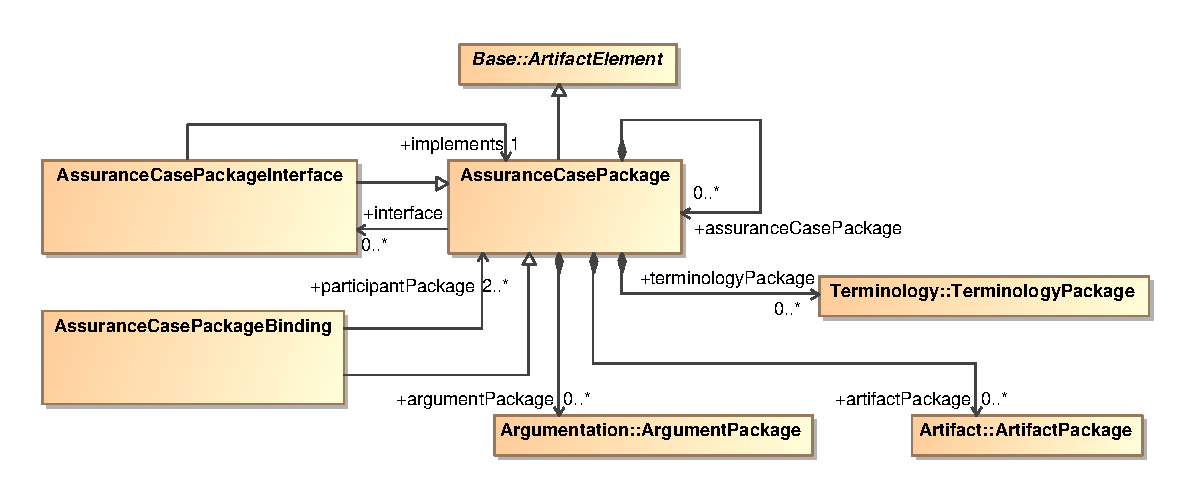
\includegraphics[width=1\linewidth]{fig/AssuranceCase.eps}
	\caption{Packages of SACM}
	\label{fig:ac}
\end{figure}

The core element in the \textit{AssuranceCase} package is the \textit{AssuranceCasePackage} element, which extends the \textit{ArtifactElement} in the \textit{Base} package. The implication is that an \textit{AssuranceCasePackage} can be considered to be an artefact. An \textit{AssuranceCasePackage} can hold a number of \textit{ArgumentPackage}s, \textit{TerminologyPackage}s and \textit{ArtifactPackage}s, which are modelled in the \textit{Argumentation}, \textit{Terminology} and \textit{Artifact} packages respectively.

Sometimes, the developer of an \textit{AssuranceCasePackage} may want to make part of the \textit{AssuranceCasePackage} public so that they can be re-used. Consider the scenario where an \textit{AssuranceCasePackage} is established with its structured argumentation in it with regard to system properties for a particular type of system. Such argumentations may be re-used by other system assurance experts (e.g. for system integration). The developer can make the argumentation public in a \textit{AssuranceCasePackageInterface}, so that the argumentation is visible externally for other developers to use.

It is often usual in the system integration process to integrate assurance cases of systems to form an overall assurance case. SACM handles this scenario with the \textit{AssuranceCasePackageBinding}, which binds two or more \textit{AssuranceCasePackageInterface}s together to form an overall \textit{AssuranceCasePackage}. This particular scenario is discussed in Section~\ref{}.

\subsection{SACM Base Package}
\label{sec:basePack}
The \textit{Base} package captures the foundational concepts of SACM, the structure of the \textit{Base} package is shown in Figure~\ref{fig:base}. The base element of all SACM elements is \textit{Element}. Its direct children are \textit{LangString}, \textit{MultiLangString} and \textit{SACMElement}.
\begin{figure}
	\centering
	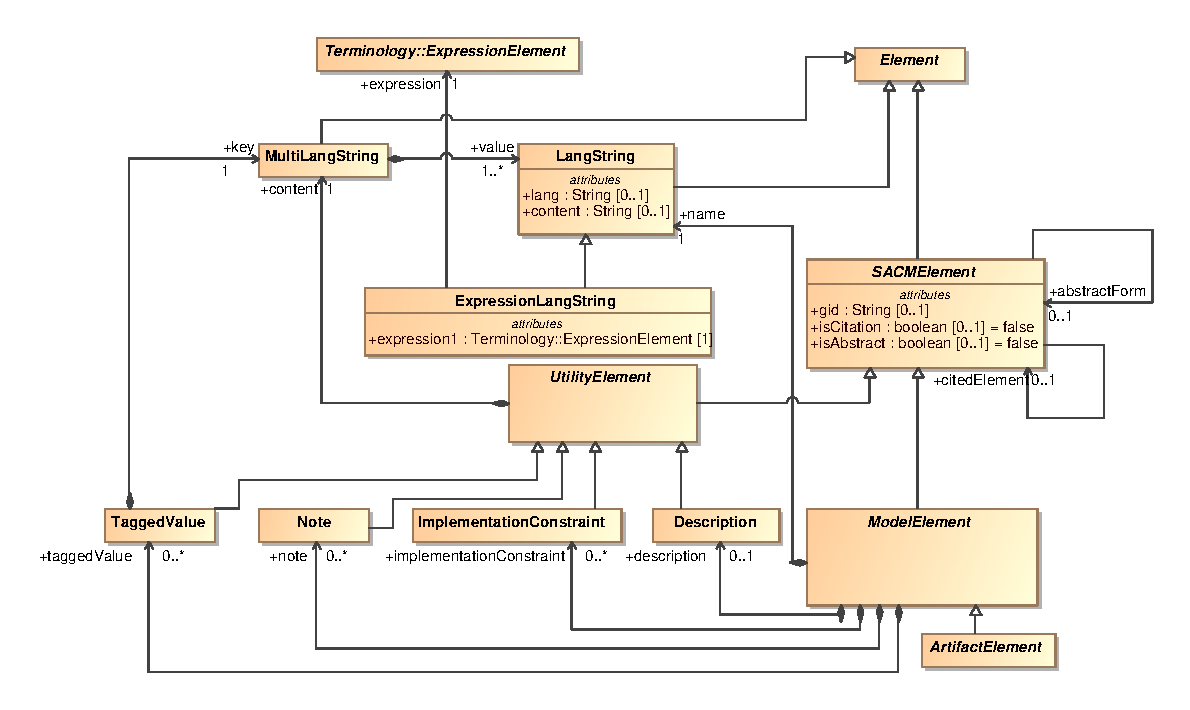
\includegraphics[width=1\linewidth]{fig/Base.eps}
	\caption{Packages of SACM}
	\label{fig:base}
\end{figure}

 \textit{LangString} is used as an equivalence to \textit{String} in broad terms, except it provides the addtional feature \textit{+lang} which allows the users to define what language is used in the \textit{LangString}. \textit{ExpressionLangString} is used to not only record a \textit{String} in SACM, but also refer to its corresponding \textit{Expression} organised in a \textit{TerminologyPackage}. The usage of \textit{ExpressionLangString} is discussed in Section~\ref{}. \textit{MultiLangString}, as its name suggests, is used to express the same semantics using different languages. For example, to express 'hazard' in both English and German, the user can create a \textit{MultiLangString} with two \textit{LangString}, like shown in Figure~\ref{fig:mulitiLang}.
\begin{figure}
	\centering
	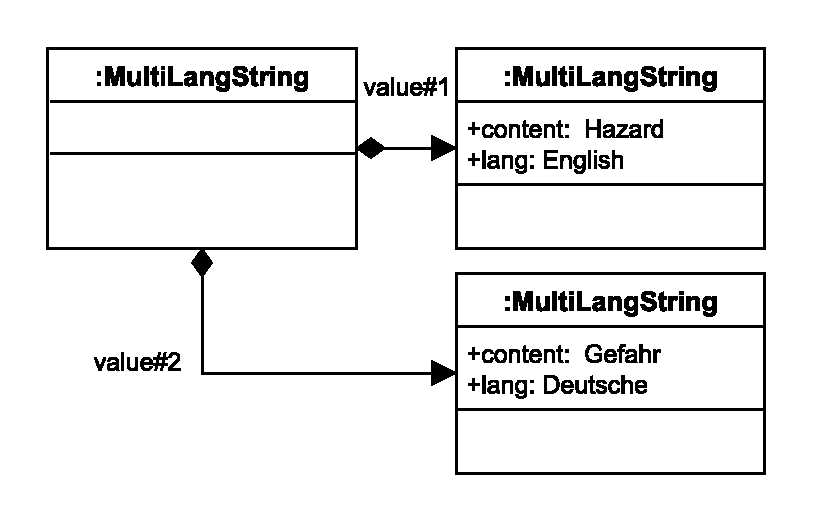
\includegraphics[width=0.5\linewidth]{fig/MultiLangString.eps}
	\caption{Packages of SACM}
	\label{fig:mulitiLang}
\end{figure}
The \textit{MultiLangString} can then be associated to other SACM elements to denote the same meaning. What is more important than multiple natural language support is the support for computer languages. We envision that in the future, system assurance can benefit from automation, by using which system assurance can be partially automated. In this case, \textit{MultiLangString} can be used to hold both natural languages and computer languages (e.g. formal languages) to support automated proving of argumentation. 

\textit{SACMElement} is an abstract element which lays the foundation of all SACM elements. \textit{SACMElement} can record a \textit{+gid}, which stands for \textit{global identification}, for each \textit{SACMElement}, within the same root \textit{Assurance Case}, should have an unique id. \textit{SACMElement} is also able to refer to (or 'cite') other \textit{SACMElement}s, which is useful for implicit references discussed in Section \ref{}. The \textit{citedElement} and \textit{isCitation} properties are used for this purpose. A \textit{SACMElement} can also be abstract, denoted by the \textit{isAbstract} property. A \textit{SACMElement} can also be an \textit{abstractForm} of another, which is discussed in Section \ref{}. 

\textit{ModelElement} further refines \textit{SACMElement} which contains a \textit{name} and a set of \textit{UtilityElement}s. A \textit{ModelElement} can contain a \textit{Description} describe its contents. Like previously mentioned, a \textit{Description} can be expressed in any language via its usage of \textit{MultiLangString}. A \textit{ModelElement} can also contain an \textit{ImplementationConstraint}, in some cases, validation rules and/or queries to models are needed for specific \textit{ModelElement}s, \textit{ImplementationConstraint} can be used to specify such constraints in computer languages (e.g. Object Constraint Language~\cite{}). A \textit{ModelElement} can also contain a number of \textit{Note}s, to hold additional information rather than descriptions. Finally, a \textit{ModelElement} can also contain a number of \textit{TaggedValue}s, which are essentially \{key, value\} pairs. \textit{TaggedValue} can be considered as an extension mechanism to allow the users to associate additional features to a \textit{ModelElement} (other than the features modelled in the current version of SACM\footnote{Version 2.0 as of April, 2018}).

The \textit{Base} package also defines the \textit{ArtifactElement}, in the sense that all elements that extend \textit{ArtifactElement} are considered to be \textit{Artifact}s. The reason for this is discussed in Section~\ref{}. 

In summary, the \textit{Base} package lays the foundation for SACM, it provides facilities not to only express assurance cases (to be precise, assurance case models) in natural language, but also in computer languages. The \textit{Base} package also provides a number of \textit{UtilityElement}s so that the user can use them to describe \textit{ModelElement}s as precisely as possible.

\subsection{SACM Artifact Package}
\label{sec:artiPack}
Before delving into the \textit{Argumentation} package, it is necessary to discuss the \textit{Artifact} package. The structure of the \textit{Artifact} package is shown in Figure~\ref{fig:arti}. 
\begin{figure}
	\centering
	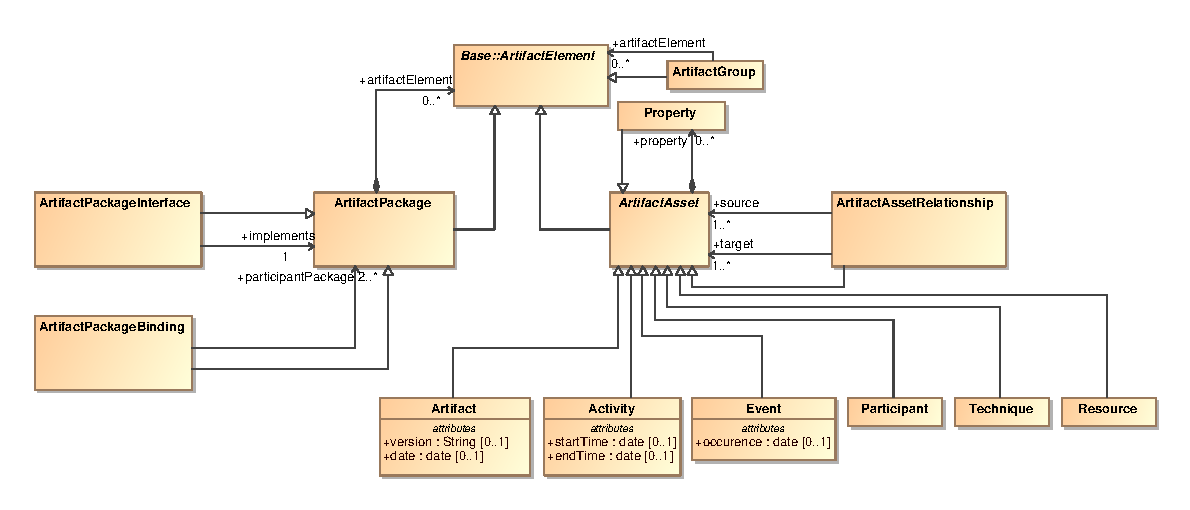
\includegraphics[width=1\linewidth]{fig/Artifact.eps}
	\caption{Packages of SACM}
	\label{fig:arti}
\end{figure}

All elements in the \textit{Artifact} package extend \textit{ArtifactElement} in the \textit{Base} package. \textit{ArtifactElement}s are organised in \textit{ArtifactPackage}s to promote modularity. SACM considers integration of assurance cases at the level of \textit{ArtifactPackage}, \textit{ArtifactPackageInterface} and \textit{ArtifactPackageBinding} are used for this purpose.

\textit{ArtifactGroup} is a new concept introduced in SACM 2.0. As \textit{ArtifactPackage} can contain rather a large number of \textit{ArtifactElement}s, the \textit{ArtifactGroup} provides the user with a means to selectively group \textit{ArtifactElement}s, so that the user of SACM can group/view \textit{ArtifactElement}s as they wish.

\textit{ArtifactAsset} allows the users to create corresponding artefact elements in SACM, it can contain a number of \textit{Property}-ies to hold user-defined properties. \textit{Artifact} is used to record a piece of information (such as hazard log, failure logic models, etc). \textit{Activity} is used to record an activity (e.g. specification of requirements). \textit{Event} is used to record an event (e.g. creation/modification of \textit{Artifact}s). \textit{Participant} is used to record participants involved in certain \textit{ArtifactAsset}. \textit{Technique} is used to record the techniques used in a particular \textit{Activity}. \textit{Resource} is used to record a piece of resource, usually in the form of some electronic file for an assurance case. And finally, \textit{ArtifactAssetRelationship} is used to link \textit{ArtifactAsset}s (e.g. connecting \textit{Activity} to \textit{Participant}s). Note that the \textit{ArtifactAssetRelationship} is a generic relationship, however, the user can choose to use \textit{Property} to specify the purpose of an \textit{ArtifactAssetRelationship}. 

One question to with respect to the \textit{Artifact} package is how to refer to external resources (such as system requirements, system design model, etc). SACM uses  

\subsection{SACM Argumentation Package}
\label{sec:argPack}
The \textit{Argumentation} Package captures the concepts required to model structured arguments regarding system properties. The structure of the \textit{Argumentation} package is shown in Figure~\ref{fig:arg}. 

\begin{figure}
	\centering
	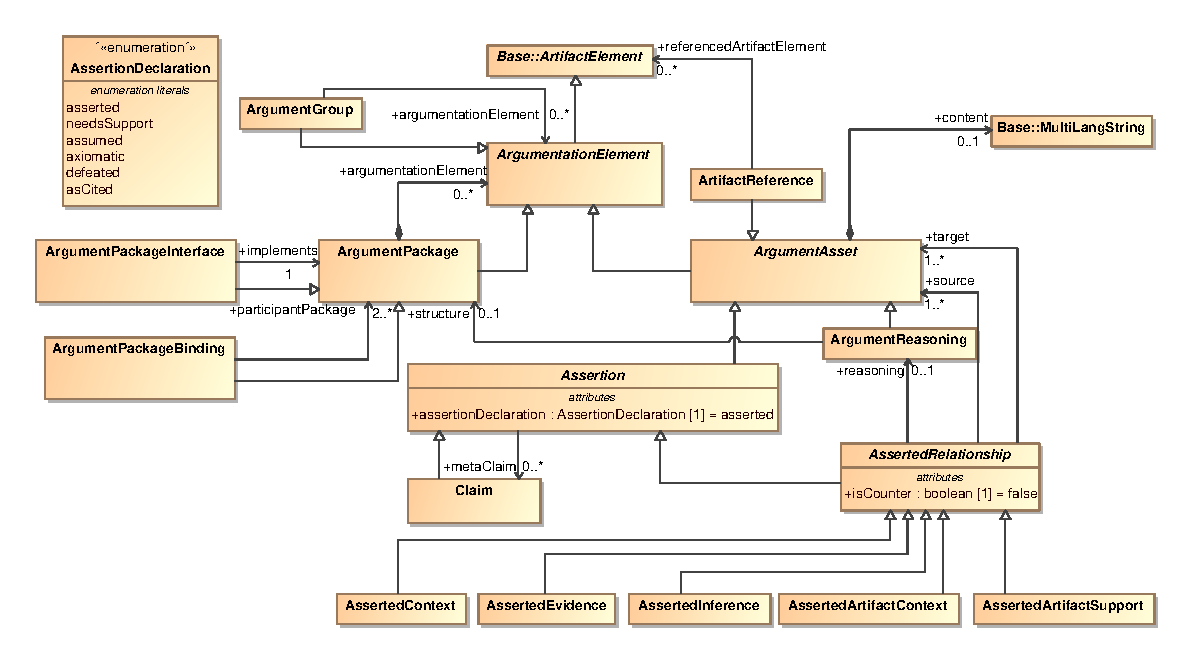
\includegraphics[width=1\linewidth]{fig/Argumentation.eps}
	\caption{Packages of SACM}
	\label{fig:arg}
\end{figure}
The root element of the \textit{Argumentation} package is the \textit{ArgumentationElement}, which is a direct child of \textit{ArtifactElement} in the \textit{Base} package. This implies that all elements in the \textit{Argumentation} package are also considered to be artifacts. 

To promote modularity, argumentations are organised in \textit{ArgumentPackage}s. \textit{ArgumentationPackage} can contain a number of \textit{ArgumentationElement}, which can either be \textit{ArgumentPackage}s (and their children) or \textit{ArgumentAsset}s. \textit{ArgumentAsset} can store a \textit{content}, as discussed in Section~\ref{sec:basePack}, the content can be in any language\footnote{via the usage of \textit{MultiLangString}}.

\textit{ArtifactReference} is a type of \textit{ArgumentAsset}, which is able to refer to an \textit{ArtifactElement} (technically, all elements in the \textit{AssuranceCase}, \textit{Argumentation}, \textit{Artifact} and \textit{Terminology} packages are \textit{ArtifactElement}s). \textit{ArtifactReference} is typically used to refer to evidence stored in the \textit{Artifact} package of an \textit{AssuranceCasePackage}.

\textit{Assertion} and its children are the elements that form the structured argumentation in the \textit{Argumentation} package. An \textit{Assertion} has an \textit{AssertionDeclaration} to distinguish different kinds of \textit{Assertion}s. The \textit{AssertionDeclaration}s are as follows: \will{I probably need to demonstrate these in examples}

\begin{itemize}
	\item \textbf{asserted} - the default declaration, means that the \textit{Assertion} is proposed and is supported by evidence;
	\item \textbf{needsSupport} - a flag indicating that the \textit{Assertion} is not supported yet (needs further development);
	\item \textbf{assumed} - a flag indicating that the truth of the \textit{Assertion} is assumed although no supporting evidence is provided;
	\item \textbf{axiomatic} - a flag indicating that the truth of the \textit{Assertion} is axiomatically true without further supporting evidence;
	\item \textbf{defeated} - a flag indicating that the truth of the \textit{Assertion} is invalidated by a counter-evidence and/or argumentation;
	\item \textbf{asCited} - when an \textit{Assertion} 'cite's another \textit{Assertion} (via the +citedElement property in \textit{SACMElement}), the truth of the \textit{Assertion} is transitively derived from the value of the cited \textit{Assertion}.
\end{itemize}

\textit{Claim} and \textit{AssertedRelationship} are the core elements of the \textit{Argumentation} package. \textit{AssertedRelationship} are used to connect \textit{ArgumentAsset}s to form structured argumentation:

\begin{itemize}
	\item \textbf{AssertedCotnext} - this relationship is used to connect contextual \textit{Claim}s to \textit{asserted} \textit{Claim}s. 
	\item \textbf{AssertedEvidence} - this relationship is used to connect evidence (referenced via \textit{ArtifactReference}) to \textit{Claim}s. 
\end{itemize}



 One typical usage of \textit{AssertedRelationship} is to connect \textit{ArtifactReference}s to \textit{Claim}s (providing evidence for an argument) using the \textit{AssertedEvidence}. 

\textit{ArgumentReasoning} is also a type of \textit{ArgumentAsset}, it is used to provide a reasoning for a particular \textit{AssertedRelationship}

\subsection{SACM Terminology Package}
\label{sec:termPack}

\begin{figure}
	\centering
	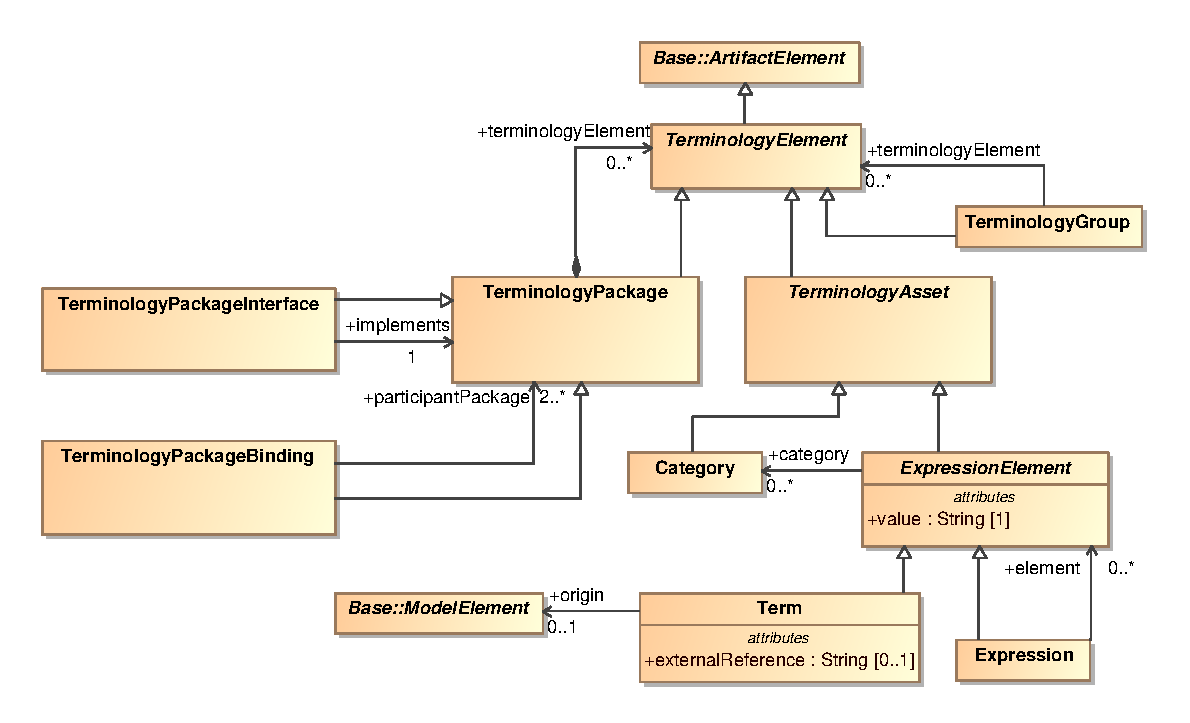
\includegraphics[width=1\linewidth]{fig/Terminology.eps}
	\caption{Packages of SACM}
	\label{fig:term}
\end{figure}

